\section{Terrain Traversal Evaluation: Versioned Extension of Experiment 2}
Six normalized collision heightfields retain the original robot, liquid, contact law, controller and actuator limits. New feature heights are at most $1.8$ mm, or $2\%$ of the $90$ mm main sphere radius. Facet slopes are below $0.03$ rad; the inherited maximum tilt remains $0.12$ rad. The unchanged twenty-six-second high-level command script is evaluated on three reset contexts. Traversal requires ordered approach, obstacle-region crossing, progress beyond its registered exit, at least $0.5$ m horizontal displacement, physical validity and route completion. A short pilot is not a traversal success.

\begin{table}[ht]\centering\caption{Versioned terrain-route outcomes; three contexts each.}\begin{tabular}{lc}\hline Terrain & Full route passes\\\hline
FLAT & 3/3\\
MILD & 3/3\\
RANDOM & 3/3\\
BUMPS & 3/3\\
SLOPES & 3/3\\
COURSE & 2/3\\
\hline\end{tabular}\end{table}
Native positions demonstrate translation rather than sphere rotation alone. Offline sphere-centre reconstruction and contact queries show approximately $1.80$--$1.83$ mm elevation gain at the bump/plateau. However, inherited compliant-contact penetration is approximately $5.4$--$5.6$ mm, exceeding the feature heights. These results therefore establish bounded traversal in the existing compliant-contact model, not hard-obstacle or hardware capability. One connected-course context encounters the ROM guard near $19.57$ s; no gain or contact sweep removes this failure.

\begin{figure}[ht]\centering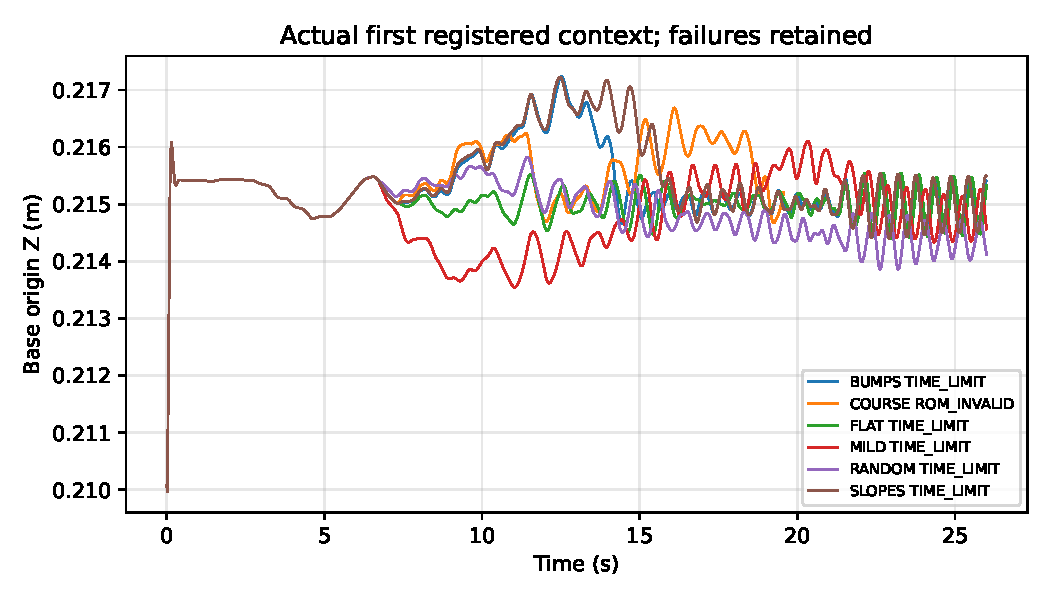
\includegraphics[width=.95\linewidth]{../upgrade/figures/height.pdf}\caption{Actual body-origin elevation on registered routes. Sphere-centre climb and initial contact settlement are audited separately.}\end{figure}

\section{Liquid Sloshing Visualization and Modeling}
The frozen liquid baseline retains one fixed component and one moving mass with two slide coordinates. The two-coordinate energy and native two-way reaction are unchanged; no second fluid load is applied. The adopted cylindrical first-mode frequency and moving mass follow linear equivalence formulas\cite{orr2021rotary}. The inherited COM-height placement and assumed damping do not establish full continuum pressure-moment equivalence.

For $k=\alpha/R$ with $J_1'(\alpha)=0$, the visualization uses
\[
\eta(x,y)=\frac{m_1}{m}\frac{kh}{J_2(\alpha)}J_1(kr)\frac{q_xx+q_yy}{r}.
\]
Its continuous mean elevation is zero, and its first volume moment matches $(m_1/m)\mathbf q$. The origin uses the removable limit. This is a derived linear surface reconstruction from equivalent modal states, not an independently validated hydrodynamic surface. MjvScene triangles and transparent wall copies do not modify native model/data physics arrays. Tests verify volume/moment identities and visualization separation. Actual XYZ trails are projected on native collision facets, not drawn on a fictitious horizontal plane.

\section{Independent Liquid Reference Feasibility}
Three new isolated-container GPU WCSPH runs use pinned Chrono10.0.0, Tait EOS, cubic kernel, Adami BCE and RK2. The $8$ mm/$50$ microsecond and $6$ mm/$50$ microsecond cases each integrate $400$ steps; a $6$ mm/$25$ microsecond pair integrates $800$, totaling $1600$ new SPH steps. The coarse twenty-millisecond screen passes, while both finer cases exceed preregistered pressure and wall-weight-force gates. Particle masses sum to approximately $0.49218$ and $0.46202$ kg, differing from the nominal $0.499$ kg ROM payload. This is a two-spacing screen with geometry/mass mismatch, not consistent spatial convergence.

The static time window is far shorter than the approximately $0.470$ s modal period. Frequency, damping, dynamic phase lag and surface errors cannot be identified. Acceleration, braking, lateral motion, tilt and recorded rough-terrain fluid replays remain gated. Actual six-degree-of-freedom tank kinematics are archived and a tested interpolator is supplied, but no unvalidated full robot--fluid coupling is opened. Modal energy and particle kinetic energy are not treated as identical observables. The overall physical-liquid status remains \texttt{SPH\_BLOCKED}; the reference is an independent numerical candidate, not experimental ground truth.

\begin{figure}[ht]\centering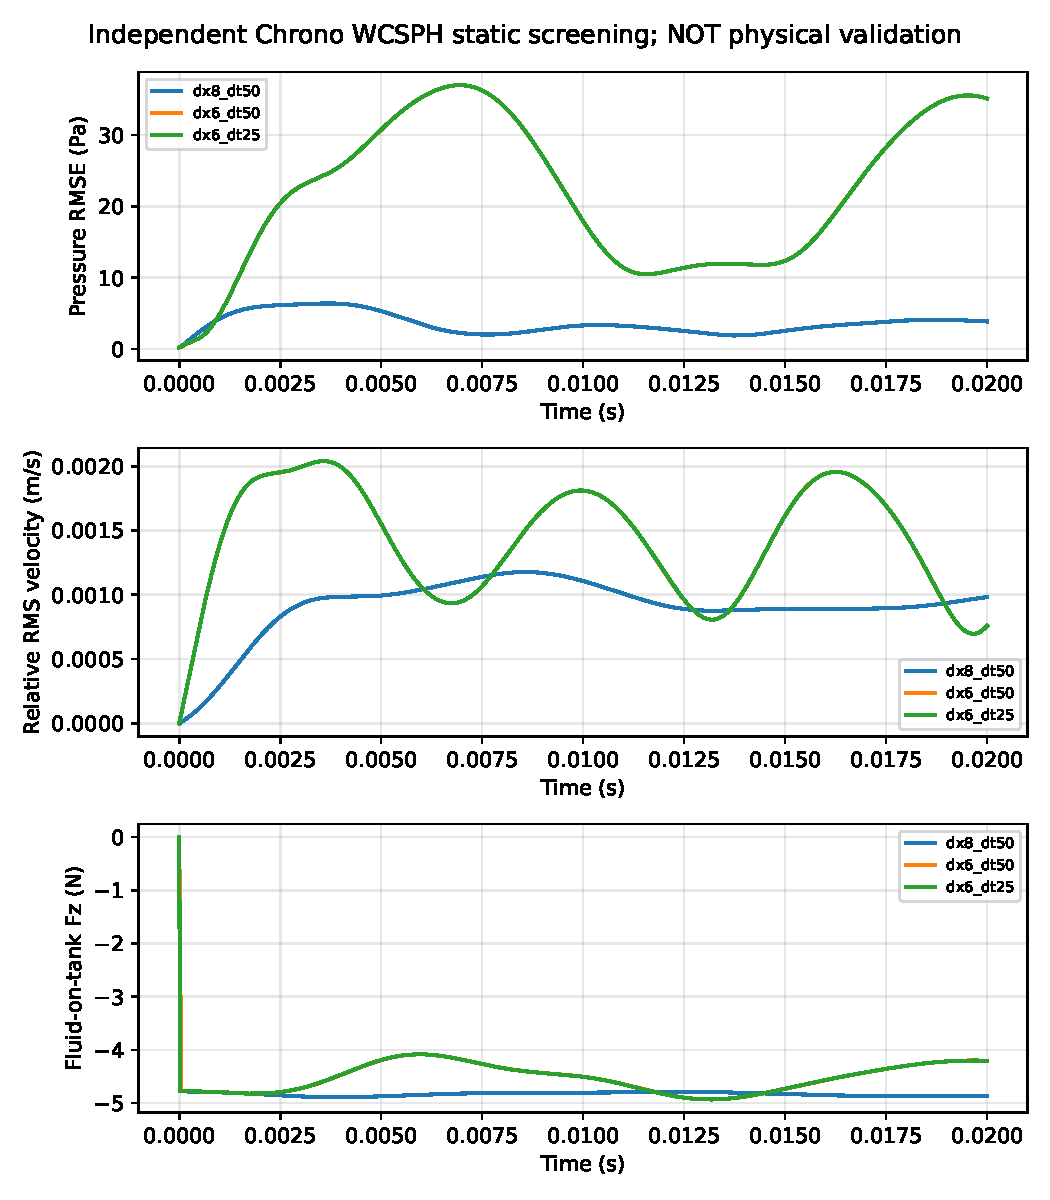
\includegraphics[width=.95\linewidth]{../research/high_fidelity/static_screen.pdf}\caption{Actual new independent GPU static screens. Completing CUDA steps does not validate the liquid model.}\end{figure}

\paragraph{Motion-quality qualification.} Geometric route completion differs from the inherited velocity/yaw-quality thresholds. A descriptive application of those unchanged thresholds yields fifteen of eighteen joint route/quality passes, including two of three bump cases and one of three connected-course cases. Motors reach the unchanged $\pm10$ Nm limits; the largest any-motor saturation fraction is about $39.4\%$. No new post-hoc saturation acceptance gate is invented, and the original Experiment1 gate remains unchanged. These headroom and tracking limitations prevent interpreting successful crossing as robust navigation.
